\hspace{0,5in}Latex merupakan system pengaturan cara pengetikan dokumen. Latex adalah perangkat lunak yang dapat di download tanpa harus membayar. Sejarahnya, Donald Knuth (Standford University) mulai mengembangkan sistem pemrosesan dokumen yang disebut "\,Tex dan Metafont" pada tahun 1977. Knut mengungkapkan bahwa Tex merupakan sistem pengetikan dengan tujuan
untuk membuat buku yang "\,cantik" , khususnya yang terdiri atas formula-formula matematis. Hingga sekarang, Latex telah berkembang dan project saat ini adalah Latex3.\par \vspace{12pt}

LaTeX merupakan word processor (pengolah kata, pembuat dokumen) mirip Microsoft Word. LaTeX lebih cocok digunakan untuk membuat dokumen yang panjang, bukan yang pendek. Dengan begitu, keampuhan LaTeX dapat ditampilkan. LaTeX juga lebih dapat menampilkan kecanggihannya ketika kita menulis scientific document.
Kelebihan menggunakan latex antara lain :
1.  Hasil tampilan dokumennya profesional sekali dengan kata lain mirip buku teks.
2.  Ketika kita ngetik, kita tidak peduli tampilan dan layout. Layout nanti diatur oleh file utama (misal: main.tex).
3.  LaTeX itu free of charge atau gratis.
4.  Rumus-rumus matematika dapat diatur dengan mudah.
5.  Tidak pernah crash (adanya error karena salah memasukkan command atau karena software tidak updated)
6.  File-nya relatif kecil.
8.  Tutorial dan command untuk symbol banyak tersedia di internet

\hspace{0,3in}Biasanya Latex digunakan untuk mengetik dokumen yang berisi formula-formula matematis. Jenis dokumen yang dihasilkan dapat berupa artikel, buku, tesis, disertasi, hingga surat bisnis maupun surat pribadi. Dokumen yang hasilkan oleh latex berbeda antara input dengan output dari MS Word atau Libre Office. Misalnya di MS Word kita mengetik "\,\$a\$" maka yang muncul di dokumen hasil adalah "\,\$a\$", sedangkan dengan input yang sama, Latex memberikan output "\,a". Karena ide dari Latex adalah membiarkan penulis menulis dokumen dan menyerahkan desain dokumen ke "\,document designer", maka hasil dari dokumen Latex akan terlihat lebih "\,cantik".\par \vspace{12pt}

\section{Instalasi LaTeX}\par \vspace{8pt}

Ada banyak editor untuk latex dan tidak semua editor sesuai dengan setiap pengguna. Semua itu tergantung pada selera masing-masing. Karena alasan ini, akan saya tunjukan bagaimana dasar-dasar latex berjalan. Banyak pengguna memilih MikTeX untuk Windows karena MikTeX sudah mempunyai semuanya yang diperlukan untuk menjalankan program latex.
\par \vspace{12pt}
\subsection{Linux}
\par \vspace{8pt}
Jika menggunakan linux, maka Anda bisa menggunakan paket texlive di beberapa repository. Setelah itu Anda bisa menggunakan berbagai macam text editor dan menjalankan file dengan format .tex dengan perintah pdflatex.
\par \vspace{12pt}
\subsection{Windows}
\par \vspace{12pt}
Langkah pertama untuk pengguna windows yaitu :

\newcounter{numberedCntC}
\begin{enumerate}
\item Install tex compiler. Tex compiler yang sering digunakan yaitu Miktex dan Texlive. Kedua perangkat lunak ini merupakan software yang paling banyak digunakan meskipun banyak perangkat lunak yang lain. Miktex yang diinstall pertama kali hanya memiliki paket dasar saja. Kemudian paket-paket tambahan lainnya dapat diinstall sesuai kebutuhan. Berbeda dengan Miktek, saat menginstall Texlive maka semua paket yang
ada akan diinstal meskipun belum tentu kita butuhkan. Sehingga instalasi Texlive lebih lama (kurang lebih 20 menit pada komputer dengan processor pentium i3 dan RAM 6 GB) daripada Miktex. Pilihan Miktex atau Texlive tergantung dari ruang hardisk yang ada, jika ruang hardisk masih banyak tidak ada salahnya menginstall Texlive. Saat ini saya menggunakan Miktex
(OS Windows) dan Texlive (Unix). Keduanya dapat didownload di Miktex website dan Texlive website (pilih salah satu).
\item Install Tex Editor. Tex editor yang tidak berbayar juga banyak. Baik di windows maupun unix, bisa menggunakan texmaker sebagai tex editor. Perangkat lunak tersebut bisa di download melalui websitenya. Didalam texmaker inilah nantinya untuk menulis dokumen latex.
\item Langkah terakhir yaitu memulai menggunakan latex. Buka texmaker, pilih file kemudian pilih new, kemudian tulis seperti contoh dibawah ini:
\setcounter{numberedCntC}{\theenumi}
\end{enumerate}

\ref{image1.jpg}:
\begin{figure}[ht]
	\centerline{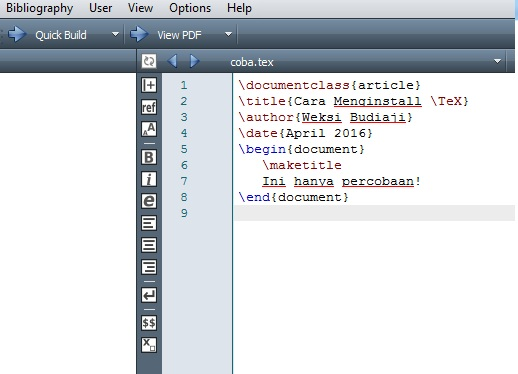
\includegraphics[width=13.54cm,height=9.78cm]{gambar/image1.jpg}}
\caption{Texmaker}
\label{image1.jpg}
\end{figure}

\begin{enumerate}
\setcounter{enumi}{\thenumberedCntC}
\item Setelah menulis file latex seperti diatas, maka save file. Misalkan save dengan nama 'coba'. Kemudian klik tanda panah "\,quick build" atau bisa dengan tekan tombol F6. Untuk melihat hasil pdf nya bisa dengan menekan tombol F7.
\setcounter{numberedCntC}{\theenumi}
\end{enumerate}

\textbf{Macam- macam Editor Latex}

\newcounter{numberedCntE}
\begin{enumerate}
\item \textbf{Emacs dengan AUCTex}
\begin{itemize}
\item OS: Windows, Mac (termasuk fork Aquamacs), Unix
\item Lisensi: Free software (GPL)
\item Bahasa: de, dk, fr, is, it, jp, nl, pl, se, sk didukung oleh AUCTeX
\item Unicode: Ya, sejak Emacs 23
\item RTL/bidirectional support: sejak Emacs 24, melalui bidi-mode
\item \% !TeX directives: Tidak, tetapi Emacs memiliki beberapa realisasi untuk file local variables
\item Syntax highlighting: Ya, bisa diatur lewat customize and Elisp
\item Code completion: Ya, via Emacs Predictive Completion, yang mendukung AUCTeX tanpa konfigurasi lebih lanjut
\item Code folding: Ya
\item Spell checking: Ya
\item SyncTeX: Ya
\item Built-in output viewer: Ya
\item Project management: org-mode, reftex-mode
\end{itemize}
\hspace{0,5in}Emacs adalah salah satu editor tertua, yang mendukung mode penyuntingan LaTeX, ConTeXt, dan Plain TeX, AUCTeX dan paket untuk mengelola kode-kode sumber, RefTeX.

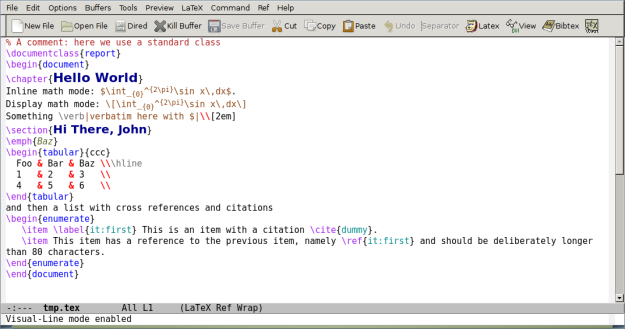
\includegraphics[width=10.95cm,height=7.87cm]{gambar/image2.jpg}
\par \vspace{12pt}

RefTeX membuat seluruh referensi Anda mudah ditemukan layaknya C-c $<$key$>$, baik untuk BibTeX maupun biblatex, dan ia memiliki pintasan (shortcut key) pula untuk bernavigasi di antara bagian-bagian dokumen dengan menggunakan C-c =: secara default.


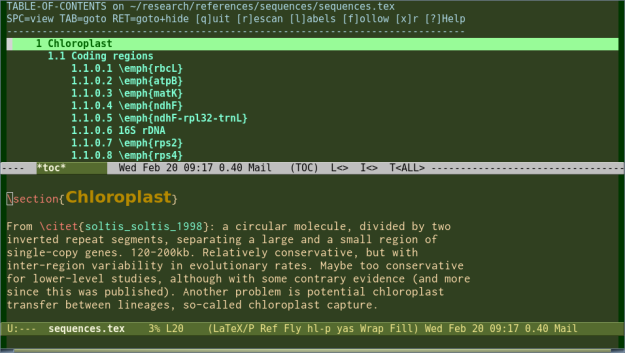
\includegraphics[width=15.64cm,height=8.83cm]{gambar/image3.jpg}

(Tema warna dapat dikonfigurasi sebebas mungkin)

AUCTeX mendukung multi-file parsing, sehingga dokumen-dokumen besar dengan perintah \textit{$\setminus$input} atau \textit{
$\setminus$include} mudah dikompilasikan dengan \textit{C-c C-c} pada berkas yang bersangkutan. Tidak perlu lagi kembali ke master file hanya untuk mengompilasi.
\par \vspace{12pt}
Fitur AUCTeX \textit{preview-latex} adalah pratayang WYSIWYG untuk rumus-rumus. Fitur-fitur terkemuka Emacs:

\begin{itemize}
\item Menggunakan table-insert bersama dengan fungsi
table-generate-source dan table-recognize-* untuk membuat tabel-tabel dengan mudah.
\item Banyak sekali shortcut key tersedia
\item Terdokumentasi dengan baik, baik Emacs itu sendiri melalui manual Emacs dan manual AUCTex Texinfo, maupun melalui banyak buku dalam beberapa bahasa.
\end{itemize}

\item \textbf{Vim dengan LaTeX-suite}
\begin{itemize}
\item OS: Windows, Mac, Linux, BSD, dan lain-lain
\item Lisensi: Open Source Charityware
\item Bahasa: ?
\item Unicode: Ya
\item RTL/bidi support: sebagian
\item \% !TEX directives: Tidak, tetapi memiliki modelines
\item Syntax Highlighting: Ya, bisa dikustomisasi
\item Code Completion: Ya (menggunakan Omni Completion, bisa diperluas dengan plugin SnipMate)
\item Code Folding: Ya
\item Spell Checking: Ya
\item SyncTeX: Ya, lihat pertanyaan ini
\item Built-in Output Viewer: Tidak
\item Project Management: ?
\item Jika Anda benar-benar kelas berat, Anda akan selalu menggunakan Vim. Ada banyak macro yang dibuat untuk Vim untuk membantu menyunting berkas LaTeX.
\end{itemize}
\begin{figure}[ht]

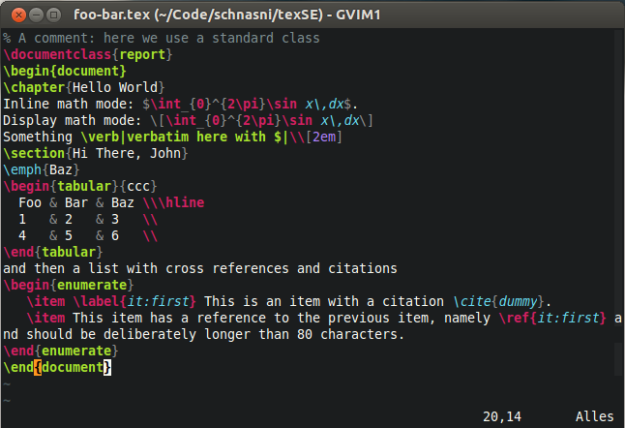
\includegraphics[width=15.57cm,height=10.66cm]{gambar/image4.jpg}
\end{figure}

Anda dapat melakukan word/command completion melalui
\begin{equation}
<C-P> dan <C-N>,
\end{equation}untuk memilih saran sebelumnya atau sesudahnya.

Ada versi Vim dengan menu-menu grafis, yang bernama gVim. Jika ia digunakan dengan Latex-suite, maka banyak perintah TeX ditampilkan di menubar untuk mempercepat penyuntingan.
\par \vspace{12pt}
\textbf{Fitur-Fitur}
\par \vspace{12pt}
Vim juga memiliki fitur code-folding, karena paket vim-late menawarkan code-folding otomatis. Folding juga bisa dilakukan secara manual berdasarkan kunci (misalnya \{\{\{ dan \}\}\}) untuk membuka dan menutup fold otomatis. Contoh folds bisa dilihat pada gambar berikut:

\begin{figure}[ht]

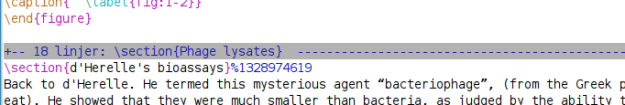
\includegraphics[width=15.12cm,height=2.54cm]{gambar/image5.jpg}
\end{figure}

Fitur Vim masih sangat banyak. Namun yang dapat dijelaskan dalam tulisan ini hanya beberapa saja, diantaranya adalah sebagai berikut:

VIM

Regex

\begin{itemize}
\item Perintah dan pintasan kibor yang powerful
\item Sangat bisa dikustomisasi
\item Smart Indenting
\end{itemize}
LaTeX-Suite

\begin{itemize}
\item Panggil cepat kompiler dengan $\setminus$ll; tayangkan hasil dengan $\setminus$lv
\item Environments dapat diakses dengan tiga huruf dalam insert mode:
\end{itemize}
\hspace{0,2in}EEQ = environment persamaan

EFI = environment gambar (figure)

\begin{itemize}
\item Place-holders ($<$+text+$>$) dapat dilompati dengan Ctrl-J tanpa meninggalkan insert mode
\item Inverse searching: klik ganda penampil PDF dan Anda lompat ke baris kode sumber tex yang bersesuaian.
\end{itemize}

\item \textbf{Texmaker - texmaker}
\begin{itemize}
\item Platforms: Windows XP/Vista/7/8, OS X 10.5+, Linux
\item License: GPL, gratis
\item Languages: cs, de, el, en, es, fa, fr, gl, hu, it, nl, pl, pt, pt (bra), ru, se, sr, zh (cn), zh (tw)
\item Unicode: Ya
\item RTL/bidi: ?
\item \% !TEX directives: Tidak
\item Syntax Highlighting: Ya, bisa dikustomisasi
\item Code Completion: Ya, bisa dikustomisasi
\item Code Folding: Ya
\item Spell Checking: Ya
\item SyncTeX: Ya
\item Built-in Output Viewer: Ya, mendukung PDF
\end{itemize}
\item \textbf{TeXworks - texworks}
\begin{itemize}
\item OS: Windows XP/Vista/7/8, OS X, Linux
\item Lisensi: GPL
\item Bahasa: en, af, ar, ca, cs, de, fa, fo fr, it, ja, nl, ko, pl, pl, ru, sl, tr zh
\item Unicode: Ya
\item RTL/bidi: Ya
\item \% !TEX directives: Ya
\item Syntax Highlighting: Ya, regex-based
\item Code Completion: Ya, bisa dikustomisasi berdasarkan daftar 'known entry'
\item Code Folding: Tidak
\item Spell Checking: Ya, tetapi harus diinstal sendiri
\item SyncTeX: Ya
\item Built-in Output Viewer: Ya, PDF (Poppler-based)
\item Project Management: Tidak
\item Di Windows dan Linux, saya menggunakan TeXworks, yang menyediakan jendela editor kode dan pratayang. Klik pada pratayang dokumen akan langsung menandai kode LaTeX yang bersesuaian.
\end{itemize}

\item \textbf{Kile - kile}
\begin{itemize}
\item OS: Linux, Windows1 (XP, Vista, 7)
\item LIsensi: GNU GPL 2
\item Bahasa:
\begin{verbatim}bg, bs, ca, cs, da, de, el, en\_GB, eo, es, et, fi, fr, ga, gl, hi, hne, hu, it, ja, kk, lt, mai, ms, nb, nds, nl, nn, pl, pt, pt\_BR, ro, ru, sk, sv, tr, ug, uk, zh\_CN, zh\_TW
\end{verbatim}
\item Unicode: Ya
\item RTL/bidi: Ya
\item \% !TEX directives: Tidak2
\item Syntax Highlighting: Ya, bisa dikustomisasi
\item Code Completion: Ya, bisa dikustomisasi
\item Code Folding: Ya
\item Spell Checking: Ya
\item SyncTeX: Ya (namun flag -synctex=1 harus ditambahkan secara manual pada build engine)
\item Built-in Output Viewer: Terbatas3 (pratayang PNG dari sebagian kode - misalnya environment yang dipilih - dikonversikan dari DVI/PS/PDF)
\item Project Management: Ya
\end{itemize}
\begin{figure}[ht]

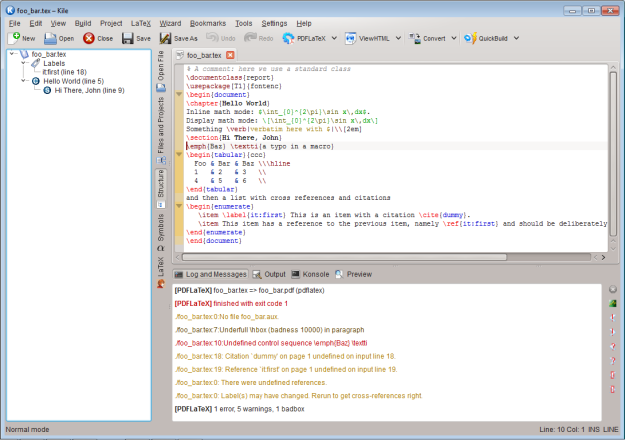
\includegraphics[width=14.76cm,height=10.39cm]{gambar/image6.jpg}
\end{figure}


\item \textbf{TeXstudio - texstudio}

\begin{table}[ht]
	\caption{Instalasi Paket}
	\centering
	\begin{tabular}{cccc}
		\hline
		No&Keterangan&\\
		\hline
		.1&OS: Windows XP/Vista/7, OS X, Linux, FreeBSD&\\
		.2&Lisensi: GPL v2&\\
		.3&Bahasa: cs, de, en, es, fr, hu, ja, pt\_BR, zh\_CN&\\
		.4&Unicode: Ya&\\
		.5&RTL/bidi: ?&\\
		.6&TeX directives: Ya&\\
		.7&Syntax Highlighting: Ya, bisa dikustomisasi&\\
		.8&Code Completion: Ya, bisa dikustomisasi dan auto-customized&\\
		.9&Unicode: Ya&\\
		.10&Code Folding: Ya&\\
		.11&Spell Checking: Ya&\\
		.12&SyncTeX: Ya&\\
		.13&Built-in Output Viewer: Ya, mendukung PDF&\\
		.14&Project Management: Ya&\\
		.15&Saya merekomendasikan TeXstudio sebagai fork yang menarik dari Texmaker yang saya rasa lebih nyaman dan bisa dikustomisasi.&\\
		\hline
	\end{tabular}
\end{table}
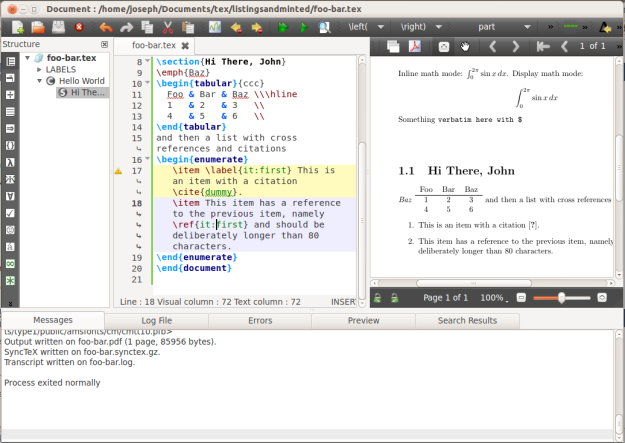
\includegraphics[width=15.23cm,height=10.79cm]{gambar/image7.jpg}

Fitur-fitur lainnya:
\begin{itemize}
\item cross-platform
\item dukungan penulisan (incremental search, folding, navigasi, auto-completion, custom macros)
\item syntax highlighting
\item inline interactive spell-checking
\item mendukung program-program LaTeX utama, termasuk tikz, pstricks, dan lain-lain
\item multi-views: math, structure
\item dukungan SVN
\item bisa berjalan via USB flash disk
\item mendukung synctex
\item termasuk penampil PDF, tetapi masih bisa dikonfigurasi untuk memakai viewer eksternal (juga dengan synctex)
\item developer dan komunitas yang sangat aktif dan responsive
\end{itemize}


\item \textbf{LyX}
\begin{itemize}
\item OS: Windows, Mac, and Linux
\begin{itemize}
\item Lisensi: Open Source
\item Sangat intuitif dan ramah pengguna, dan bisa impor/ekspor ke LaTeX.
\item Terlalu banyak ftur untuk disebutkan, paling bagus: Jika Anda ingin menulis rumus matematika "\,2-dimensional", LyX cocok untuk itu.
\end{itemize}
\end{itemize}
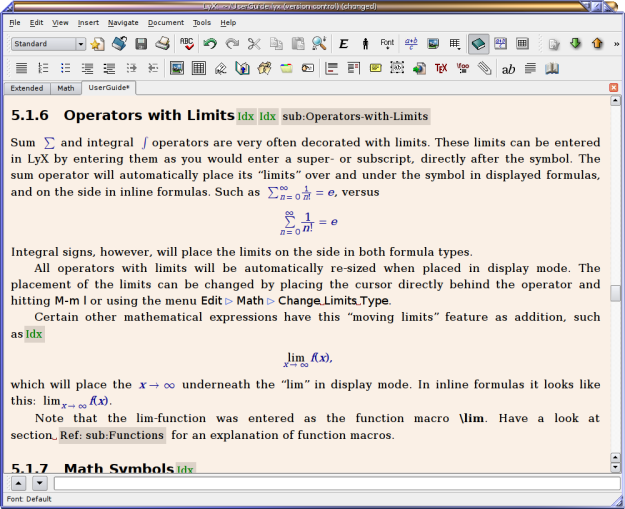
\includegraphics[width=14.10cm,height=11.48cm]{gambar/image8.jpg}

\item \textbf{Sublime Text dengan LaTeX Plugin}
\setcounter{numberedCntE}{\theenumi}
\hspace{0,2in}OS: Windows, Mac, Linux

Sublime Text merupakan salah satu editor yang sederhana tetapi tetap powerful. Sublime Text mirip Notepad++, namun tersedia dalam berbagai macam platform dan sangat mudah diatur untuk LaTeX dengan plugin LaTeXTools atau LaTeXing, keduanya tersedia dari Package Control. Sublime juga mirip dengan TextMate, tetapi dikembangkan lebih aktif dan memiliki komunitas yang lebih besar yang menyediakan plugin-nya. Sublime juga lebih cantik daripada keduanya.
\par \vspace{12pt}

Hal yang perlu Anda perhatikan bahwa Sublime Text adalah software berbayar, dan akan meminta lisensi selama periode evaluasi (seharga USD 70). Anda memungkinkan untuk dapat menjalankan Sublime Text tanpa membeli lisensi, tetapi Anda akan terus diingatkan bahwa Anda menggunakan salinan yang belum diregistrasikan.
\par \vspace{12pt}


Sublime Text memiliki peralatan atau fitur-fitur canggih untuk mengetik, sehingga dapat membuat lebih nyaman dan memudahkan pekerjaan Anda:

\begin{itemize}
\item multiple cursors
\item go-to ke mana saja
\item snippets
\item incremental find
\item manajemen proyek
\item build-systems yang banyak
\end{itemize}
Dan masih banyak lagi (lihat Perfect Workflow in Sublime Text 2). ScreenShot di bawah juga menampakkan fiturnya untuk menemukan sitas-sitasi (citations) dari BibTeX.
\par \vspace{12pt}

Sublime Text ini editor yang hampir sempurna, dengan potensi yang hampir tidak terbatas. Daftar fiturnya panjang sekali. Instal Package Manager, dan paket-paket tambahan dari repositori bisa dipasang dalam beberapa detik saja.

\begin{itemize}
\item OS: Windows, Unix
\item Lisensi: Free to try, free to buy
\item \% !TEX directives: Ya
\item Syntax highlighting: Ya
\item Code completion: Ya
\item Code folding: Ya
\item Spell check: Ya, baik built-in maupun dengan plugin
\item SyncTeX: Ya
\item Built-in output viewer: Tidak
\item Project management: Ya
\end{itemize}
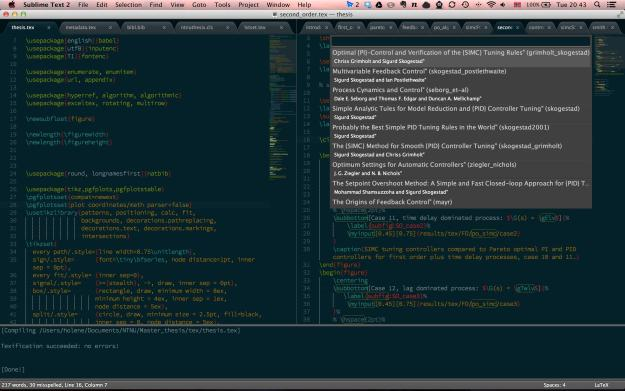
\includegraphics[width=15.67cm,height=9.80cm]{gambar/image9.jpg}

\item \textbf{TeXlipse}
\begin{itemize}
\item OS: Windows, Mac, Linux and others (Java based)
\item Lisensi: Open Source
\end{itemize}
Saya telah berbahagia menggunakan TeXlipse di Eclipse sejak lama, ia memiliki code completion terintegrasi (termasuk entri-entri BibTeX), template-template yang mudah dikustomisasi, panel outline, dan secara langsung ia terintegrasi dengan Eclipse itu sendiri yang secara otomatis memiliki shortcuts, version control, dan lain-lain.
\par \vspace{12pt}

Kemudian ada plugin penampil PDF yang digunakan untuk Eclipse, software tersebut bernama Pdf4 Eclipse. Dengan dukungan SyncTeX, yang mendukung pencarian maju/mundur di dalam dokumen LaTeX. Karena TeXlipse me-rebuild kode-kode LaTeX secara otomatis (di background) setelah sekali disimpan, maka kode dan pratayang dari dokumen selalu disinkronkan.

\item \textbf{Gummi}
\begin{itemize}
\item OS: Linux (tersedia versi unstable untuk Windows)
\item Lisensi: Open Source
\end{itemize}


Emacs memang bagus, tetapi yang seringkali saya pakai adalah Gummi. Ia memiliki panel pratayang yang sangat berguna untuk mengetahui kesalahan sintaks dan kesalahan format sesegera mungkin. Dan ketika Anda menyimpan dokumen LaTeX ia akan menyimpan PDF secara otomatis. Fitur lainnya termasuk peralatan bantuan penulisan matriks, memasukkan gambar, dan
sitasi (citation).
\par \vspace{12pt}

\begin{figure}[ht]

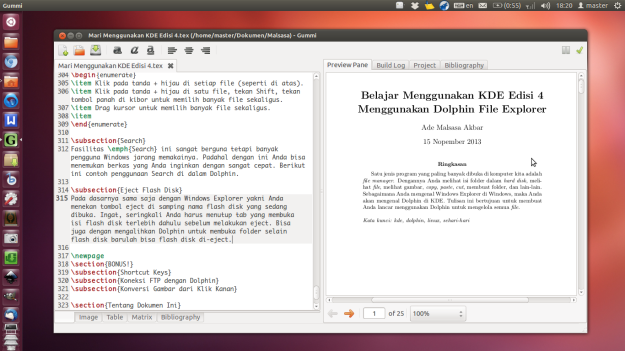
\includegraphics[width=15.45cm,height=8.68cm]{gambar/image10.jpg}
\end{figure}

\item \textbf{LaTeXila}
\begin{itemize}
\item OS: Linux
\item Lisensi: Open source
\item Unicode: Ya
\end{itemize}
\hspace{0,5in}LaTeXila adalah lingkungan LaTeX yang terintegrasi untuk GNOME. Ia memiliki antarmuka yang bagus dan jelas. LaTeXila tersedia pada Ubuntu Software Center. Anda dapat melihat preview dari apa yang Anda tulis kapanpun Anda mau.
\par \vspace{12pt}

LaTeXila memiliki komentar-komentar "\,ajaib" untuk membuat todonotes, yang akan tayang di panel struktur di sebelah kiri. Komentar itu adalah \%TODO dan \%FIXME, yang harus diikuti oleh teks (jika tidak ada teks, maka tidak ada yang tayang di panel).

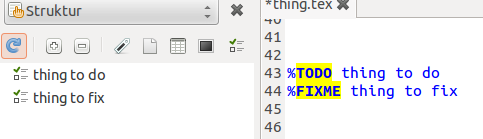
\includegraphics[width=12.78cm,height=3.68cm]{gambar/image11.jpg}


\item \textbf{Geany with GeanyLaTeX}
\begin{itemize}
\item OS: Windows, Mac, Linux dan lain-lain
\item Lisensi: Open Source
\end{itemize}
\end{enumerate}


Editor bagus lainnya adalah Geany. Software ini memiliki plugin untuk LaTeX. Plugin ini di-maintain oleh salah satu developer utama Geany sendiri. Plugin ini memiliki wizard untuk dokumen LaTeX baru, autocompletion, insert environment dengan mudah, dan tentu terdokumentasi dengan baik.

